\section{Project Management \& Development Tools}
    \subsection{Obstacles in the development process}
    \begin{frame}[t]{Project Management \& Development Tools}\framesubtitle{Tasks we need to solve}
        \begin{itemize}
        	\item Version Control
        	\item Code Review
        	\item Wiki
        	\item Documentation
        	\item Continuous Integration
        	\item Artifact Repository
        \end{itemize}
    \end{frame}
    \subsection{Tools}
    \begin{frame}[t]{Project Management \& Development Tools}\framesubtitle{Version Control}
        \begin{itemize}
            \item Git
        	\begin{itemize}
        		\item Foundation of workflow
                \item Powerfull
                \item Easy to make mistakes
        	\end{itemize}
        \end{itemize}
    \end{frame}

    \begin{frame}[t]{Project Management \& Development Tools}\framesubtitle{Code Review, Wiki}
        \begin{itemize}
        	\item Phabricator
        	\begin{itemize}
        		\item Archanist
                \begin{itemize}
                    \item Uses git
                    \item Interfaces with Phabricator
                    \item Unit tests \& linting
                \end{itemize}
        		\item Web interface
                \begin{itemize}
                    \item Hub for the entire multi project
                    \item User story and task management
                    \item Wiki
                    \item Code review
                \end{itemize}
        	\end{itemize}
        \end{itemize}
    \end{frame}
    \begin{frame}[t]{Project Management \& Development Tools}\framesubtitle{CI, Documentation, Artifact Repo}
        \begin{itemize}
        	\item Jenkins
        	\begin{itemize}
        		\item Gradle
                \begin{itemize}
                    \item DevOps
                \end{itemize}
                \item Automated Testing
        		\item Artifactory
                \item Javadoc
        	\end{itemize}
        \end{itemize}
    \end{frame}
\section{Architecture}
    \begin{frame}[t]{Architecture}\framesubtitle{Old GIRAF architecture}
        \only<1>{%
        \begin{figure}
        	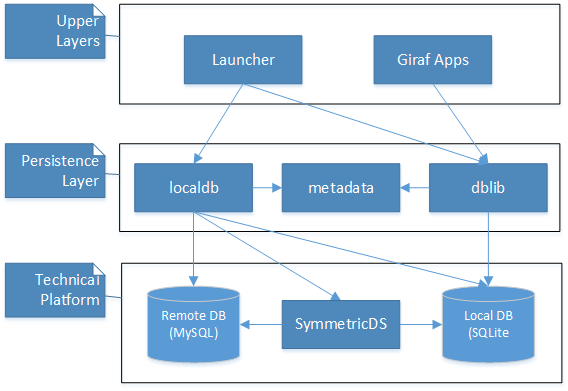
\includegraphics[width=0.8\textwidth]{images/old_architecture.png}
        \end{figure}}
        \only<2>{%
        \begin{figure}
        	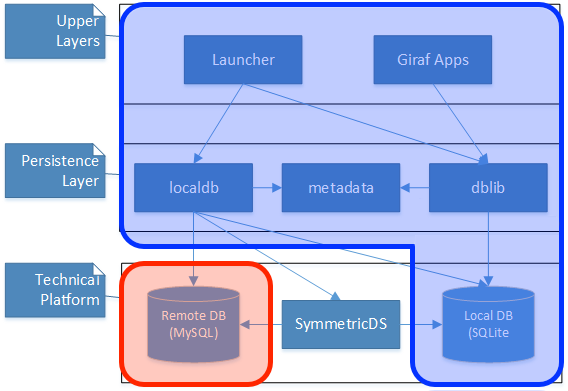
\includegraphics[width=0.8\textwidth]{images/old_architecture_memes.png}
        \end{figure}}
    \end{frame}

    \begin{frame}[t]{Architecture}\framesubtitle{New GIRAF architecture}
    	\begin{figure}
    		\scalebox{0.6}{%
        	\pgfdeclarelayer{background}
\pgfsetlayers{background,main}
\tikzstyle{double_arrow}=[latex'-latex']
\tikzstyle{component}=[draw, fill=blue!20, text width=8em,
text centered, minimum height=2.5em]
\tikzstyle{client_comp}=[draw, fill=blue!20, text width=4em,
text centered, minimum height=2.5em]
\tikzstyle{client_comp_synca}=[draw, fill=blue!20, text width=4em,
text centered, minimum height=1.5em]
\tikzstyle{bgbox}=[fill=green!20, rounded corners, draw=GoogleGrey, dashed]
\begin{tikzpicture}[auto]

    %%%%%%%%%%%%%%%%%%%%%%%%%%%%%%%%%%%%%%%%%%%%%%%%%%%%%%%%%%%%%%%%%%%%%
    % REST API                                                          %
    %%%%%%%%%%%%%%%%%%%%%%%%%%%%%%%%%%%%%%%%%%%%%%%%%%%%%%%%%%%%%%%%%%%%%
    \node[component] (persistence) {Persistence};
    \node[component, above = 0.6cm of persistence] (service) {Service};
    %core
    \path (persistence.south -| persistence.east)+(1,0) node (core_a) {};
    \path (service.north -| service.east)+(2,0) node (core_b) {};
    \path[draw, fill = blue!20] (core_a) rectangle (core_b);
    \path ($ (core_a) !.5! (core_b) $) node (core) {Core};

    %REST API background box
    \begin{pgfonlayer}{background}
        % Compute a few helper coordinates
        \path (service.west |- service.north)+(-3,+0.5) node (rest_a) {};
        \path (core_a)+(+2,-0.5) node (rest_b) {};
        \path [bgbox] (rest_a) rectangle (rest_b);
        \node [below = 0.5em of rest_a, anchor = west, inner sep = 0.5em]{REST API};
    \end{pgfonlayer}

    %Awwowwwws
    \draw [<-, dashed] ($(service.south)+(+0.1,0)$) -- ($(persistence.north)+(+0.1,0)$);
    \draw [->]     ($(service.south)+(-0.1,0)$) -- ($(persistence.north)+(-0.1,0)$);
    \draw [->]     (service) -- node {uses} (service -| core_a);
    \draw [->]     (persistence) -- node {uses} (persistence -| core_a);

    %%%%%%%%%%%%%%%%%%%%%%%%%%%%%%%%%%%%%%%%%%%%%%%%%%%%%%%%%%%%%%%%%%%%%
    % Storage                                                           %
    %%%%%%%%%%%%%%%%%%%%%%%%%%%%%%%%%%%%%%%%%%%%%%%%%%%%%%%%%%%%%%%%%%%%%
    \node[component, below = 1.5cm of persistence] (db) {Database};

    \draw [<-, dashed] ($(persistence.south)+(+0.1,0)$) -- ($(db.north)+(+0.1,0)$);
    \draw [->]     ($(persistence.south)+(-0.1,0)$) -- ($(db.north)+(-0.1,0)$);

    %storage background box
    \begin{pgfonlayer}{background}
        % Compute a few helper coordinates
        \path (db.west |- db.north)+(-3,+0.5) node (db_a) {};
        \path (core_a |- db.south)+(+2,-0.5) node (db_b) {};
        \path [bgbox] (db_a) rectangle (db_b);
        \node [below = 0.5em of db_a, anchor = west, inner sep = 0.5em]{Storage};
    \end{pgfonlayer}

    %%%%%%%%%%%%%%%%%%%%%%%%%%%%%%%%%%%%%%%%%%%%%%%%%%%%%%%%%%%%%%%%%%%%%
    % Web 'n' client                                                    %
    %%%%%%%%%%%%%%%%%%%%%%%%%%%%%%%%%%%%%%%%%%%%%%%%%%%%%%%%%%%%%%%%%%%%%
    \node[draw, cloud, cloud puffs=12, cloud ignores aspect, minimum width=9em, minimum height=5em,fill=blue!20, above = 1cm of service](web) {Internet};
    \draw [<-, dashed] ($(web.south)+(+0.1,0)$) -- ($(service.north)+(+0.1,0)$);
    \draw [->]     ($(web.south)+(-0.1,0)$) -- ($(service.north)+(-0.1,0)$);

    % CLIENT GALORE
    \node[client_comp, above = 2cm of web](client2) {$\text{App}_{2}$};
    \node[client_comp_synca, below = 0.3cm of client2] (client2_synca) {S.A.};
    \draw [<-, dashed] ($(client2.south)+(+0.1,0)$) -- ($(client2_synca.north)+(+0.1,0)$);
    \draw [->]     ($(client2.south)+(-0.1,0)$) -- ($(client2_synca.north)+(-0.1,0)$);
    \draw [<-, dashed] ($(client2_synca.south)+(+0.1,0)$) -- ($(web.north)+(+0.1,0)$);
    \draw [->]     ($(client2_synca.south)+(-0.1,0)$) -- ($(web.north)+(-0.1,0)$);

    \node[client_comp, left = 0.2cm of client2](client1) {$\text{App}_{1}$};
    \node[client_comp_synca, below = 0.3cm of client1] (client1_synca) {S.A.};
    \draw [<-, dashed] ($(client1.south)+(+0.1,0)$) -- ($(client1_synca.north)+(+0.1,0)$);
    \draw [->]     ($(client1.south)+(-0.1,0)$) -- ($(client1_synca.north)+(-0.1,0)$);
    \draw [<-, dashed] ($(client1_synca.south)+(+0.1,0)$) |- ($(web.west)+(0,+0.1)$);
    \draw [->]     ($(client1_synca.south)+(-0.1,0)$) |- ($(web.west)+(0,-0.1)$);

    \node[right = 0.2cm of client2] (client_dot){$\cdots$};

    \node[client_comp, right = 0.2cm of client_dot](clientn) {$\text{App}_{n}$};
    \node[client_comp_synca, below = 0.3cm of clientn] (clientn_synca) {S.A.};
    \draw [<-, dashed] ($(clientn.south)+(+0.1,0)$) -- ($(clientn_synca.north)+(+0.1,0)$);
    \draw [->]     ($(clientn.south)+(-0.1,0)$) -- ($(clientn_synca.north)+(-0.1,0)$);
    \draw [<-, dashed] ($(clientn_synca.south)+(+0.1,0)$) |- ($(web.east)+(0,-0.1)$);
    \draw [->]     ($(clientn_synca.south)+(-0.1,0)$) |- ($(web.east)+(0,+0.1)$);

    %clients background box
    \begin{pgfonlayer}{background}
        % Compute a few helper coordinates
        \path (service.west |- client1.north)+(-3,+0.5) node (clients_a) {};
        \path (core_a |- clientn_synca.south)+(+2,-0.5) node (clients_b) {};
        \path[bgbox] (clients_a) rectangle (clients_b);
        \node [below = 0.5em of clients_a, anchor = west, inner sep = 0.5em]{Clients};
    \end{pgfonlayer}

\end{tikzpicture}
}
        \end{figure}
    \end{frame}
